\documentclass{article}
\usepackage[utf8]{inputenc}
\usepackage{mathtools}
\usepackage{amssymb}
\usepackage{graphicx}
\usepackage{listings}
\usepackage{float}
\usepackage{gensymb}
\usepackage{amsthm}
\usepackage{longtable}
\usepackage{adjustbox}
\usepackage{physics}

\theoremstyle{definition}
\newtheorem{definition}{Definition}
\newtheorem{theorem}{Theorem}
\newtheorem{example}{Example}
\newtheorem{lemma}{Lemma}
\newtheorem{proposition}{Proposition}

\title{Quantum Computation}
\author{quinten tupker}
\date{October 8 2020 - \today}

\begin{document}

\maketitle

\section*{Introduction}

These notes are based on the course lectured by Professor Richard Jozsca in
Michaelmas 2020. Due to the measures taken in the UK to limit the spread of
Covid-19, these lectures were delivered online. These are not meant to be an
accurate representation of what was lectures. They solely represent a mix of
what I thought was the most important part of the course, mixed in with many
(many) personal remarks, comments and digressions... Of course, any
corrections/comments are appreciated.

This course is meant to be a second course on quantum computation. In
particular, all the prerequisite knowledge is covered in Cambridge's Part II
Quantum Information and Computation course. Lecture notes for this course can be
found online.

Now, to start describing course content. Quantum Computation studies algorithms
that can be run on quantum computers. Although they have yet to be implemented
in practice (but are definitely being developed at a rapid pace), and in
particular how they differ with classical computation. A remarkable result, is
that at least superficially, quantum algorithms appear to be more powerful than
classical algorithms, although it remains unclear if this is definite fact, or
if it simply easier for humans to solve complex problems using quantum
algorithms instead of classical algorithms. This is remarkable in many ways in a
philosophical sense, but here we focus on how to take advantage of these
changes. As such, we will begin with a review and extension of one of the most
famous quantum algorithms, which is Schur's factoring algorithm.

\section{Schur's Algorithm Revisited and the Hidden Hidden Subgroup Problem}

Schur's factoring algorithm finds a factor for an arbitrary number $N$. It does
not perform a complete factorisation. It merely computes a factor, which of
course can be repeated arbitrarily to get a complete factorisation, but that is
not the point here. The complexity of such an algorithm is typically measured in
terms of the number of digits of $N$, which we may denote $n = \ln(N)$. In these
terms Schur's algorithm is $O(n^3)$, which means it is ``efficient''
(computationally feasible) or

\begin{definition}[efficient algorithm]
  An algorithm is efficient if it runs in polynomial time, which generally means
  it is considered doable in practice.
\end{definition}

By comparison, the fastest known classical algorithm runs in
$O(e^{n^{1/3}\ln(n)^{1/3}})$.

Anyways, here is an outline of Schur's algorithm:

\begin{enumerate}
\item choose $a < N$ such that $(a, N) = 1$ (coprime). This can be done
  efficiently, since the probability of $a$ being coprime is fixed, and we can
  quickly calculate the GCD using Euclid's algorithm. Then consider $f(x) =
  a^x (\text{mod} N)$.
\item Use quantum algorithms to calculate the period of the this function
  (so we have converted a factoring problem into period finding). Since $a$
  is coprime, it is guaranteed to be periodic.
\item compute the factor using number theory
\end{enumerate}

The crucial component here is the period finding, which cannot be done
efficiently using a classical algorithm. So let's review quantum period finding.
Also, note that as usual, quantum oracles are implemented as unitary operators
by converting $f : \mathbb{Z}_M \to \mathbb{Z}_N$ to $U_f \ket{x} \ket{0}
\mapsto \ket{x} \ket{f(x)}$. Then, if $f$ has period $r$ (unknown), and $f$ is
one-to-one on every period, then period finding can be done using

\begin{enumerate}
\item make $\frac{1}{\sqrt{M}} \sum_0^{M - 1} \ket{i}\ket{0}$
\item apply $U_f$
\item measure the output register to get
  $$ \frac{1}{\sqrt{A}} (\ket{x_0} + \ket{x_0 + r} + \dots + \ket{x_0 + (A -
    1)r}) \ket{f(x_0)} $$
  Now the next step is the tricky part, and really is what uses the ``quantum
  magic'' here, and that involves the use of the Quantum Fourier Transform
  (QFT). [This ends lecture 1]
\item We then apply the QFT, which maps $\ket{k} \mapsto \sum_{y = 0}^M e^{xy}
  \ket{y}$, which, after some calculation (use $\sum e^{2\pi kx/y} =
  y\delta_{xy}$) leaves us with
$$ \text{QFT} \ket{\text{per}} = \sqrt{A / M} \sum_{k = 0}^{r - 1} \omega^{x_0 k
M/r} \ket{k M / r} $$
\item Making a measurement we get $C = k_0 M / r$, so $\frac{k_0}{r} =
  \frac{C}{M}$. If $k_0, r$ are coprime, we are done, since we can reduce
  $\frac{C}{M}$ to simplest terms (use Euclid's algorithm to cancel out the
  gcd). Now, number theory tells us that the probability of being coprime is
  finite and shrinks slowly (as $O(1 / \log \log (M))$), and so we can just
  repeat until we get the right period. Since $f$ is one-to-one on each period,
  it is easy to check if our period is correct.
\end{enumerate}

I feel that just being able to check if the period is correct is a somewhat lame
reason to require that the function be one-to-one on each period, but
improvements although not difficult, would complicate this explanation.

Anyways, let's see if we can motivate the Quantum Fourier Transform a bit
better. The challenge we face is that our state, $\ket{R}$ takes the form

$$ \ket{R} = \sum_k a_k \ket{x_0 + kr} $$

for an arbitrary $x_0$. In other words, we have an arbitrary shift that we want
to ignore some how. How do we do that? A natural way to spot ``things that
ignore shifts'' would be to define the shhift operator

$$ U \ket{x} = \ket{x + 1 \text{ mod } M} $$

and then, how do we say, ``we don't care about '' $U$? We look for the
eigenvectors of $U$, which are by definition, the states least affected by $U$.
Fortunately, $U$ is a permuatation matrix, so unitary, so is a quantum gate.
Then, the eigenbasis of $U$ is what we may call the set of shift-invariant
states $\chi_k$. If we write $R$ in terms of this basis we are bound to get a
state of the form

$$ \sum_k a_k \lambda_k^{x_0} \ket{\chi_k} $$

where $\mathbb{P}(k) = |a_k \lambda_k^{x_0}|^2 = |a_k|^2$ since as eigenvalues
of a unitary matrix, $|\lambda_k| = 1$ always. So as expected, probabilities are
preserved (this is not that crucial - but it's important they don't differ that
much). Anyways, important is that this transformation allows us to express our
state as a sum of multiples of the period, which is what we want.

All that remains is to find this basis, and the operation that expresses them in
terms of it. As eigenvectors of a unitary matrix are orthogonal, all we need to
do is zip the eigenvectors into a matrix. These eigenvectors are just of the
form $e^{2\pi i k l/ M}$, so we get the Quantum Fourier Transform we expect.
[End of lecture 2]

\subsection{The Hidden Subgroup Problem (HSP)}

The hidden subgroup problem asks
the question how can we find subgroup $K$ of group $G$ (this course only
considers finite $G$) given a function $f : G \to X$ that is an invertible
function of the left cosets of $K$. Our goal is to solve this problem in
$O(poly(\ln(|G|)))$.

Examples of this include Schur's algorithm where we have $G = \mathbb{Z}_p^*$,
then $K = {0, r, 2r, \dots}$, and then $f$ used before works for our purpose.
Another example is calculating \textbf{discrete logarithm}, which if done
efficiently could break encryption methods. This involves calculating logarithms
on $\mathbb{Z}_p^*$, so given $x$ finding $y$ such that for group generator $g$,
$x = g^y$. To formulate this as an HSP consider

\begin{align*}
  f : \mathbb{Z}_{p - 1} \times \mathbb{Z}_{p - 1} &\to \mathbb{Z}_p^* \\
  (a, b) &\mapsto g^ax^{-b} = g^{a - yb}
\end{align*}

where we can see that $f(a_1, b_1) = f(a_2, b_2)$ iff $(a_2. b_2) - (a_1, b_1) =
\lambda (y, 1)$ some $\lambda$. So using $K = \{\lambda (y, 1) | \lambda \in
\mathbb{Z}_{p - 1}\}$ works.

Those both involve abelian groups, but a big area of interest is solving
the problem for non-abelian groups. Examples of such problems include finding
the Automorphism group of a graph. For graph $A$ this means finding
$\text{Aut}(A)$ a subgroup of the group of permutations of the vertices of $A$
such that the overall structure (edges) are preserved. This can be formulated
quite naturally into an HSP by taking $X$ to be the set of all $n$ vertex
graphs, and then to consider the function $f_A(\pi)$ which applies permutation
$\pi$ to $A$. Clearly the result depends only on the coset of $\text{Aut}(A)$.

Even more famous is the \textbf{Graph Isomorphism} problem (GI), which is to
check whether or not two labelled graphs are isomorphic (so whether there exists
a permutation turning one into the other). This can be converted into an HSP,
although the process is more complicated. There also exists few good classical
algorithms, although in 2017 someone found an algorithm doing it in
quasi-polynomial time. 

But how far will we get with quantum algorithms. The abelian case has been fully
solved, but unfortunately the non-abelian case (which the above two problems
belong to) remains an important unsolved problem in the field. [End of lecture 3]

Briefly, another example of an HSP involving the Dihedral group is how to
calculate the shortest vector within a lattice. No good quantum algorithm exists
to solve this problem.

Now, let's develop the formalism to describe the quantum algorithm to solve the
hidden subgroup problem for any finite abelian group. Contrary to my
expectations, we jump straight into representation theory. Well, that is not
really contrary to my expectations, but I had imagine it would be more natural
to look at the problem as permutations, and to define invariant states from
there. Apparently, while it is not mentioned, it does not seem to be the central
approach thought of here.

Instead we rely on the fact that for a finite abelian group, all representations
can be seen as one dimensional representations $\chi : G \to S^1$, the unit
circle embedded in the complex plain. Being one dimensional they are all
irreducible, and also satisfy the following three properties:

\begin{itemize}
\item $\chi(g) = e^{2\pi i k / |G|}$ some $k \in \mathbb{Z}$
\item $\langle \chi_i, \chi_j \rangle = \frac{1}{|G|} \sum_{g \in G} \chi_i(g)
  \chi_j^*(g) = \delta_{ij}$
\item There are exactly $|G|$ distinct such representations, which we may label
  $\chi_g$
\item the restriction of an irreducible representation to a subgroup is also
  irreducible
\end{itemize}

A particular application of this is that \textbf{trivial representation}
$\chi_0(g) = 1$ is orthogonal to all other representations, so in general
$\sum_g \chi_k(g) = 0$. This will be helpful later on. Also, note that since
this is an abelian group, we will use $+$ to denote the group operation.

Now the crucial advantage that the abelian case has over the non-abelian case is
that all elements commute, meaning in particular that all representations can be
simultaneously diagonalised, which means a universal shift invariant state
exists. In particular, we notice that

$$ \ket{\chi_k} = \frac{1}{\sqrt{|G|}} \sum_{g \ in G} \overline{\chi_k(g)}
\ket{g} $$

Here the complex conjugate is really just convention, but it makes things look
similar to Schur's algorithm. Here it is easy to see that the eigenvalues of a
shift by $g$, denoted $U(g)$ is $U_k(g) \ket{\chi_k} = \chi_k(g) \ket{\chi_k}$.

The Quantum Fourier Transform (QFT) then as expected swaps the standard unit
basis with the shift invariant basis meaning that $QFT \ket{\chi_g} = \ket{g}$
so considering components approrpiately, and transposing to get the inverse we
find

$$ QFT \ket{g} = \frac{1}{\sqrt{|G|}} \sum_{k \in G} \chi_k(g) \ket{k} $$

Now, since we can classify all finite abelian groups as the product of cyclic
groups, the following result on representations of such groups is quite valuable

\begin{example}
For $G = \mathbb{Z}_M$, $\chi_a(b) = e^{2 \pi i ab / M}$ describes all
representations of $G$. Even better is that for $G = \mathbb{Z}_{m_1} \times
\dots \times \mathbb{Z}_{M_r}$, $\chi_{a}(b) = e^{2\pi i (a_1b_1 / M_1 + \dots +
  a_r b_r / M_r)}$. Furthermore, in this case

$$ QFT_G = QFT_{M_1} \otimes \dots \otimes QFT_{M_r} $$
\end{example}

Now let's start to truly describe the HSP algorithm for finite abelian groups.
Here we are given oracle $f:G \to K$ and we work on state space
$\mathcal{H}_{|G|} \otimes \mathcal{H}_{|K|}$

\begin{enumerate}
\item form the state space $ \frac{1}{\sqrt{|G|}} \sum_{g \in G} \ket{g}\ket{0}$
\item Apply $U_f$ for form $\frac{1}{\sqrt{|G|}} \sum_{g \ in G} \ket{g} \ket{f(g)}$
\item measure second register to get $\ket{g_0 + K}$ where $\ket{K} =
  \frac{1}{\sqrt{|K|}} \sum_{k \in K} \ket{k}$. 
\item Apply QFT and measure to get some state $\chi_g$. Note that here $g$
  does not depend on $g_0$ due to the QFT, which is the strength of this
  algorithm. [End of lecture 4] From here we can identify representations that
  become trivial when restricted to $K$ since we see that
  \begin{align*}
    QFT \ket{K}
    &= \frac{1}{\sqrt{|G||K|}} \sum_{l \in G} \left( \sum_{k \in K} \chi_l(k) \right) \ket{l} \\
    &= \sqrt{\frac{|K|}{|G|}} \sum_{l \in G \text{ st } \chi_l|_K \text{ is trivial}} \ket{l}
  \end{align*}
  using the fact that $\sum \chi_l(k)$ is either $|K|$ or 0 depending on whether
  or not $\chi_l$ becomes trivial.
\end{enumerate}

That ends the quantum part of the algorithm, where one essentially identifies
the representation $\chi_g$ that is irreducible on $G$ but that becomes the
trivial representation when restricted to $K$. This is enough to find the
subgroup of interest.

\begin{example}
  For example, one can show that if $K$ has generators $k_1, \dots, k_M$ for $K
  = O(\ln(|K|)) = O(\ln(|G|))$ then if we repeat the algorithm $O(\ln(|G|))$
  times we can find the generators (so the subgroup) with probability $> 2/3$.
\end{example}

\begin{example}
  In the $G = \mathbb{Z}_{M_1} \times \dots \times \mathbb{Z}_{M_r}$, one can
  find that finding the group is equivalent to solving a set of linear
  equations.
\end{example}

Now what goes wrong in the non-abelian case? Essentially two things can break
down. Firstly, we might not be able to implement the quantum fourier transform
in an efficient way. Secondly, because elements don't commute, we cannot
simultaneously (block) diagonalise the basis into a set of shift-invariant
states. This means one cannot fully recover the representations as one might
wish. It has nevertheless been proven when the subgroup is normal, one can solve
this efficiently (Hallgren, Russel, Ta-Shma 2003 SIAM J Comp The Hidden Subgroup
Problem and Quantum Computation Using Group Representations), and that in fact,
even in the most general non-abelian case the information we deduce is
sufficient to find $K$, however there is no efficient way to deduce $K$ from the
information we can gain using the more coarse-grained approach here (Ettinger,
Hoyer and Knill, Hidden Subgroup States are Almost Orthogonal) (so query
complexity is not high, but deducing the right information from it is high).
[End of lecture 5]

\section{Quantum Phase Estimation}

The next problem/aglorithm we discuss is \textbf{Quantum Phase Estimation} which
is how to find an eigenvalue $e^{2\pi i \phi}$ of eigenstate $\ket{v_\phi}$ of
an arbitrary unitary operator $U$. To do so we need the controlled operator
$c-U$ such that $c-U \ket{0} \ket{\xi} = \ket{0}\ket{\xi}$ and $c-U \ket{1}
\ket{\xi} = \ket{1} U \ket{\xi}$.

Now the issue is that we cannot actually contruct $c-U$ given $U$ if we only
have one of its eigenstates. If we have a full implementation, for example in
the form of a circuit, we could simply replace every gate with a controlled
gate, and that would do the job, however, if we just have a black box operator,
there is an ambiguity that arises from the fact that we may consider $U$ and
$e^{\i\alpha} U$ to be same operator. If so we find that

$$ c-e^{i\alpha} U (\ket{0} + \ket{1}) \ket{\xi} = \ket{0} \ket{\xi} +
\ket{1} e^{i\alpha} U \ket{xi} $$

so these differ by a relative phase, meaning the operator $c-U$ is truly
different from $c-e^{i\alpha} U$ despite $U$ and $e^{i \alpha}U$ being the
``same''. To resolve this, it turns out it is sufficient as long as we have one
extra eigenstate $\ket{\alpha}$ with eigenvalue $e^{i\alpha}$, since then we can
implement the algorithm as follows:

\begin{figure}[H]
  \centering
  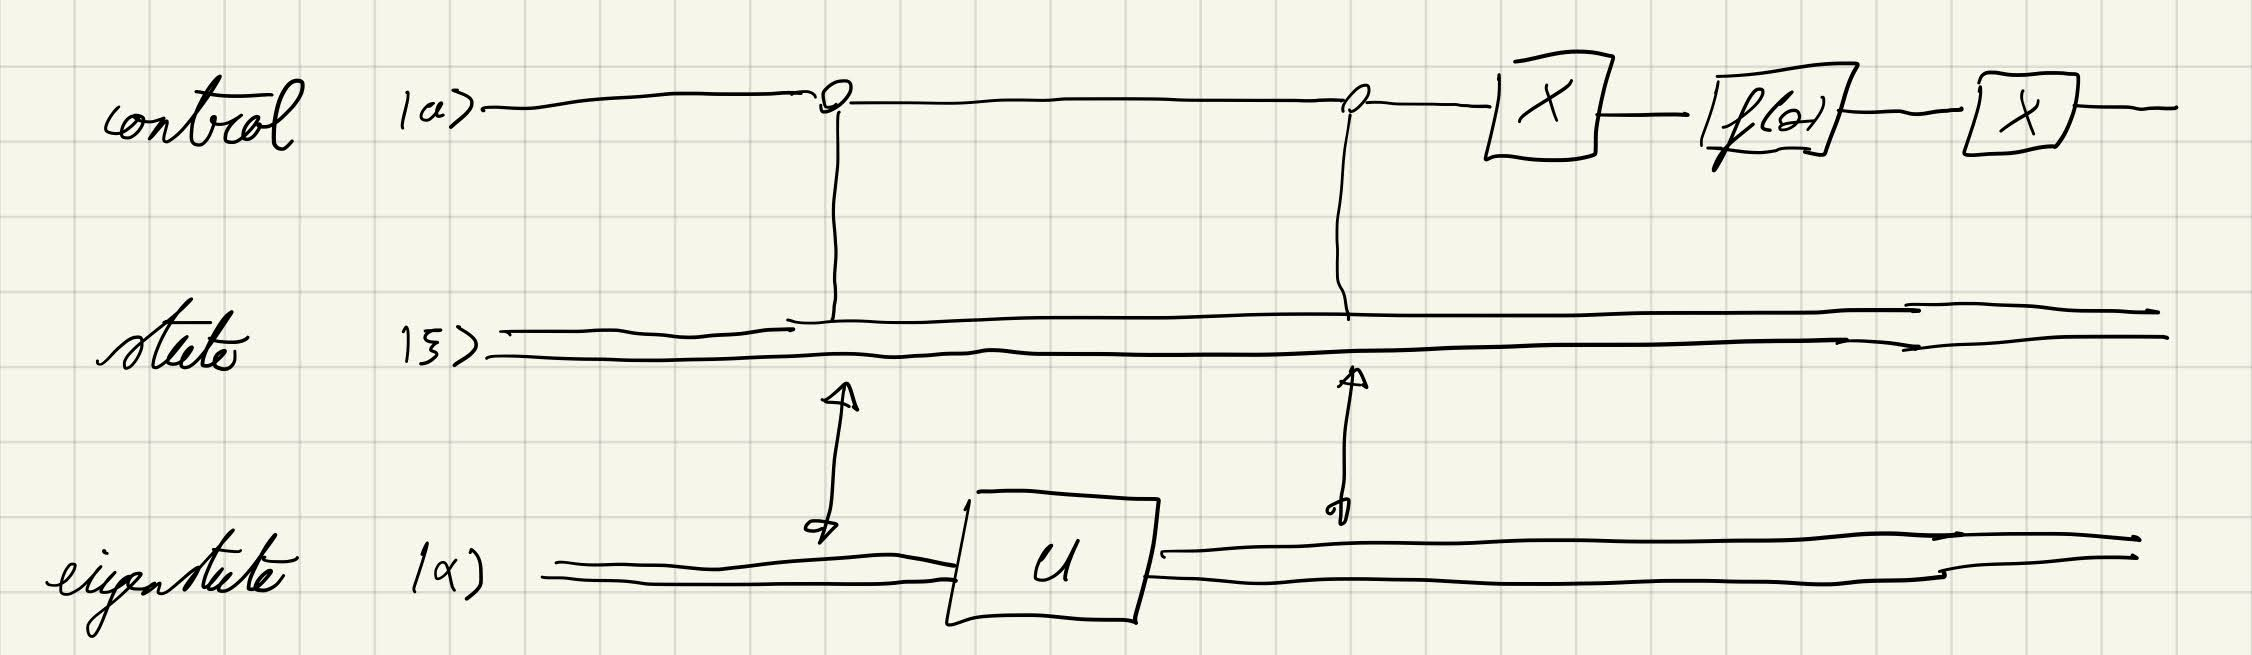
\includegraphics[width=12cm]{res/QC/controlled_U}
  \caption{Controlled $U$}
  \label{figure: controlled_U}
\end{figure}

Here the circle with the arrows indicate controlled swap operations between
$\ket{\alpha}$ and $\ket{\xi}$, double lines indicate an arbitrary
$k$-qubit state, while a single line denotes a single qubit state. $X$ denotes
the swap operator between $\ket{0}$ and $\ket{1}$ and $f(\alpha)$ denotes the
matrix

$$
\begin{pmatrix}
  1 & 0 \\
  0 & e^{i \alpha}
\end{pmatrix}.
$$

Considering case-by-case we then find that

\begin{itemize}
\item when the control is $\ket{0}$ we get $e^{i\alpha - i\alpha} \ket{0} \ket{\xi}$.
\item when the control is $\ket{1}$ we get $\ket{1} \ket{\xi}$
\end{itemize}

(typo in the picture, $\theta$ should be $-\alpha$). Now for our actual
algorithm we don't need $c-U$ instead we need (what I'll call) $N-U$ which takes
the form $N-U\ket{x}\ket{\xi} = \ket{x} U^x \ket{\xi}$. This can be implemented
as seen below for decimal expansion $x = x_{n-1} \dots x_1 x_0$.

\begin{figure}[H]
  \centering
  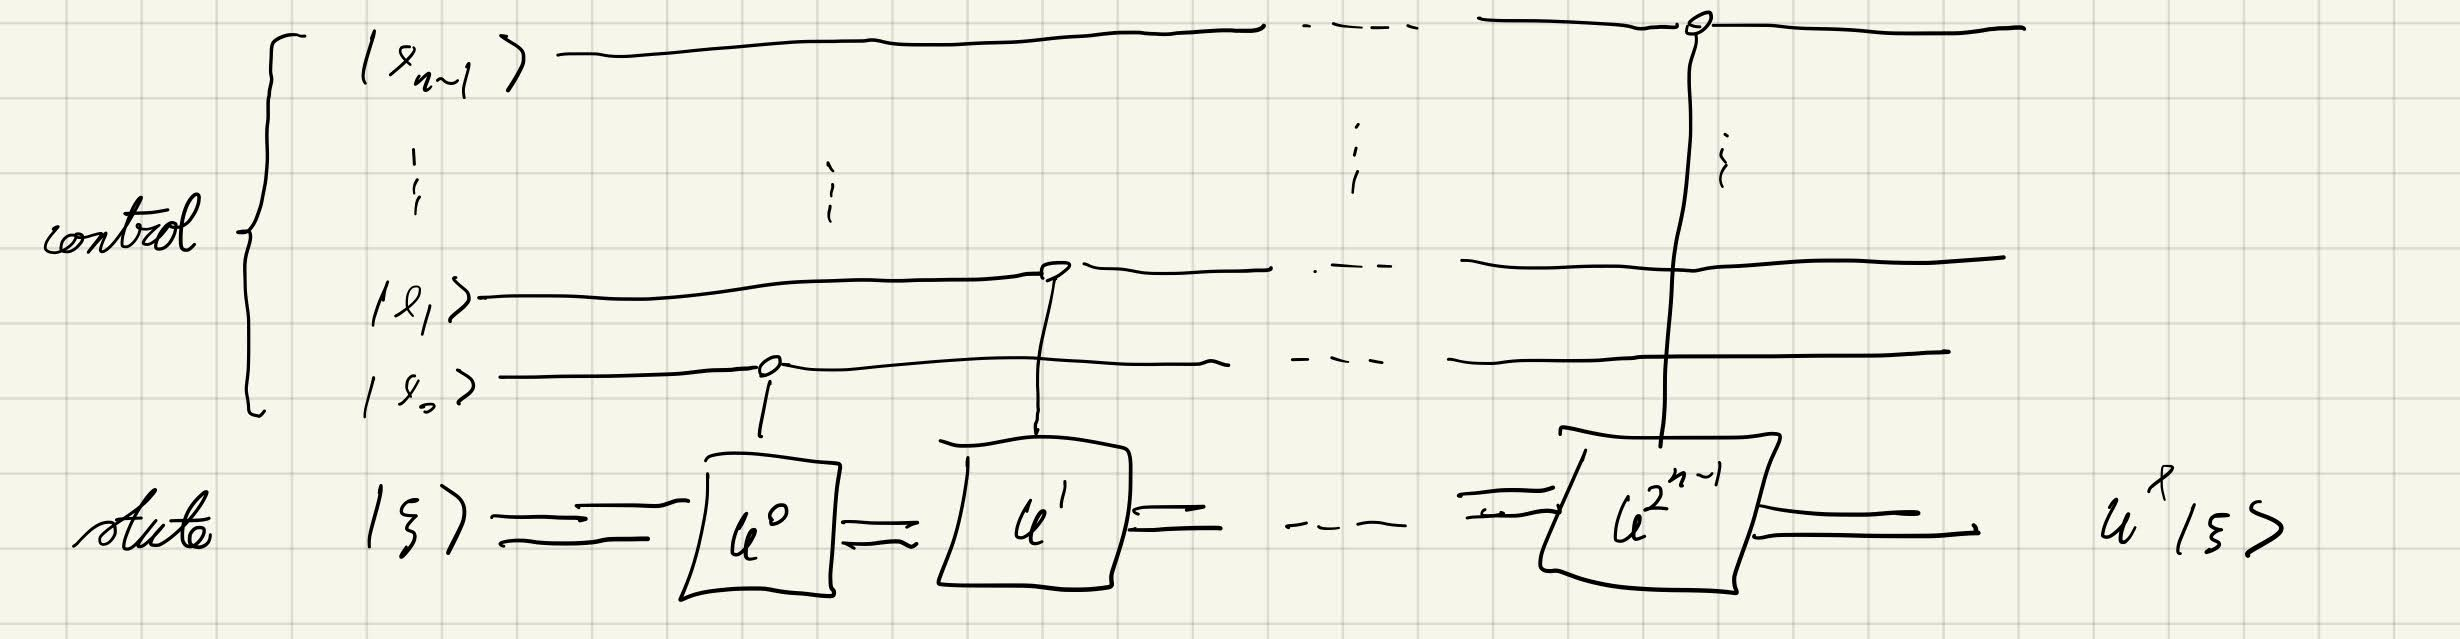
\includegraphics[width=12cm]{res/QC/generalised_controlled_U}
  \caption{Generalised Controlled $U$}
  \label{figure: generalised_controlled_U}
\end{figure}

Now that we've implemented that, the actual quantum phase estimation algorithm
is quite easy to implement:

\begin{enumerate}
\item start with $\ket{+}\ket{v_\phi}$ for $\ket{+} = H^n \ket{0}$
\item apply $N-X$ to get $\frac{1}{2^{n/2}} \sum_x e^{2\pi i \phi x} \ket{x} =
  \ket{A}$.
\item Apply $QFT^{-1}_{2^n}$ and measure to get $y_{n-1}\dots y_1y_1$. Our
  estimate for $\phi$ the is
$$ \phi \approx 0.y_0 \dots y_{n - 1} $$
\end{enumerate}
    
This is exact if $\phi = k / 2^n$ some $0 \leq k < 2^n, k \in \mathbb{Z}$. If
it's not, we have the following handy result

\begin{theorem}
  If the algorithm yields estimate $\theta \approx \phi$ then
\begin{itemize}
\item the probability of $\theta$ being the estimate to $\phi$ that is
  closest possible to $\phi$ in binary is at least $4 / \pi^2 \approx 0.4$.
\item $\mathbb{P}(|\phi - \theta| \geq \epsilon) \leq \frac{1}{2^{n +
      1}\epsilon}$.
\end{itemize}
\end{theorem}
    
In particular, we notice that if we want at least $m$ bit accuracy with
certainty $1 - \eta$ then we should run the algorithm with $n$ bits such that $n
= m + \log_2(1 / \eta)$. It is interesting here, to me, that the quantity $n$ is
sum of the desired accuracy $m$ and the chance of that accuracy (expressed in
binary) $\log_2(1/\eta)$. The fact these are equivalent in a sense is curious.
[End of lecture 6]

\begin{proof}
  First note that
  $$ QFT^{-1} \ket{A} = \frac{1}{2^n} \sum_y \sum_x e^{2\pi i (\phi - y / 2^n)x}
  \ket{y} $$
  So in particular, the probability of observing the value $y$ is
  $$ \mathbb{P}(y) = \frac{1}{y^{2n}} \left| \sum_x e^{2 \pi i (\phi - y / 2^n)}
  \right|^2 = \frac{1}{2^{2n}} \left| \frac{1 - e^{2\pi i \delta(y)}}{1 - e^{2\pi
          i \delta(y)}} \right|^2 $$
  where $\delta(y) = \phi - y / 2^n$. We use the following estimates to
  establish bounds on this quantity. Firstly, $|1 - e^{i\alpha}| = 2|\sin(\alpha
  / 2) \geq \frac{2}{\pi} |\alpha| $ if $|\alpha| < \pi$ and $|1 - e^{i \beta}|
  \leq \beta$ which can both be seen geometrically.

  Then for our first estimate, by bounding appropriately we see that

  $$ \mathbb{P}(y) \geq \frac{1}{2^n} \left( \frac{2^{n + 1} \delta(y)}{2\pi
      \delta(y)} \right)^2 = \frac{4}{\pi^2} $$
  as required.

  Our other estimate is a bit trickier. We see that

  $$ \mathbb{P}(y) \leq \frac{1}{2^{2n}} \left( \frac{2}{4\delta(y)} \right)^2 \leq
  \frac{1}{2^{2n + 2} \delta(y)^2} $$

  But we now also have to sum over all $y$ such that $|\delta(y)| > \epsilon$.
  To do so we see that in general $\delta(y)$ takes the form $\delta(\gamma) =
  \delta_\pm + k / 2^n$ meaning that $|\delta(y)| \geq \epsilon + k / 2^n$, so

  $$ \mathbb{P}(|\delta(\gamma) \geq \epsilon) \leq 2 \sum_{k=0}^\infty
\frac{1}{2^{2n + 2} (\epsilon + k / 2^n)^2} \leq \frac{1}{2} \int_0^\infty
\frac{1}{(2^n \epsilon + k)^2} dk = \frac{1}{2^{n + 2}\epsilon} $$
as required.
\end{proof}

Now a few remarks. Firstly, if $c-U^{2^k}$ is implemented as $(c-U)^{2^k}$ then
this algorithm is exponentially slow, however, for some special $U$, such as
simple exponentiation $a \mapsto a^p$ this can be done in polynomial time.
Secondly, if we apply the unitary part $U_{PE}$ to an arbitrary state, we get a
superposition in terms of eigenstates, but when we make a measurement, the
estimate for every eigenstate is good. It is just that it is random which
eigenstate we are actually measuring.

This second perspective is handy, as we can now express getting $m$ digits
correct with probability $1 - \eta$ as

$$ U_{PE} \ket{\xi} = \sqrt{1 - \eta} \ket{\phi_j} + \sqrt{\eta} \ket{\phi_\perp} $$

where $\phi_j$ are all states with $m$ correct digits, and $\phi_\perp$ are the
incorrect states.

Finally, we note that Dr Jorza, in his notes, also describes how one might
implement a quantum fourier transform in an arbitrary dimension (not necessarily
a power of two) using quantum phase finding.

\section{Amplitude Amplification}

Our next algorithm we look at is a generalisation of the essence of Grover's
search algorithm. For such, we start with some notation. We use $P_A$ to denote
projection onto the linear space $A$ which if spanned by orthogonal basis
$\alpha_i$ can be calculated as $P_A = \sum_i \ket{\alpha_i}\bra{\alpha_i}$. We
can then write a reflection as $I_A = I - P_A$. Finally, we note for convenience
that for any unitary $U,$ $UI_AU^\dagger = U_{UA}$ [End of lecture 7].

\subsection{Grover's Algorithm}

We begin by reviewing Grover's algorithm (which can be found in more detail in
the part II notes of the course). Here we are given a function

$$ f(x) =
\begin{cases}
  1 & x = x_0 \\
  0 & \text{else}
\end{cases} $$

and are trying to find $x_0$. This is an unstructured search really, and closely
relate to $NP$ complexity in classical complexity theory via the Boolean
satisfiability problem. Now, to run this algorithm we define the \textbf{Grover
  rotation} $Q = -H_n I_{\ket{0}} H_n I_{\ket{x_i}} = -I_{\ket{\psi_0}}
I_{\ket{x_0}}$. The result we rely on, but we do not prove here in particular is
that

\begin{theorem}
  $Q$ is a rotation on the space spanned by $\ket{\psi_0}, \ket{x_0}$ by angle
  $2 \alpha$ where $\sin(\alpha) = \frac{1}{\sqrt{N}}$
\end{theorem}

We then proceed to run the algorithm via

\begin{enumerate}
\item Form the uniform state $\ket{\psi_0}$ (using Hadamard gates)
\item Apply $Q$ $m$ times where
$$ m = \frac{\arccos(1 / N)}{2 \arcsin(1 / N)} = \frac{\beta}{2 \alpha} \approx
\frac{\pi}{4} \sqrt{N} $$
where $\beta$ is the angle between $\ket{\psi_0}$ and $\ket{x_0}$ and the
approximation applies when $N$ is big.
\item Measure the state to get $\ket{x_0}$ with high probability $\cos^2(\alpha)
  \approx 1 - \frac{1}{N}$.
\end{enumerate}

As we can see, this runs in $O(\sqrt{N})$ queries to the oracle. It also does
something that a classical computer is not capable of, since in particular for
$N = 4$ this is deterministic and requires exactly one query, which cannot be
matched classically.

\subsection{Returning to Amplitude Amplification}

Amplitude amplification is a generalisation of Grover's algorithm. In
particular, if we use $G$ to denote the ``good'' subspace of $\mathcal{H}$ then
see that $\forall \ket{\psi} \in \mathcal{H}, \exists \theta \in \mathbb{R},
\ket{g} \in G, \ket{b} \in G^\perp, \ket{\psi} = \sin(\theta) \ket{a} +
\cos(\theta) \ket{b}$. If we then apply $Q = -I_{\ket{\psi}} I_G$ where we
assume that $I_G$ can efficiently implemented then

\begin{theorem}
  The \textbf{Amplitude Amplification Theorem} states that $Q$ is the rotation
  $$
  \begin{pmatrix}
    \cos(2\theta) & -\sin(2\theta) \\
    \sin(2\theta) & \cos(2\theta)
  \end{pmatrix}
  $$
  in the $\ket{g}, \ket{b}$ basis.
\end{theorem}

\begin{proof}
  algebra...
\end{proof}

Using this we can greatly improve the probability of seeing $\ket{g}$. In
particular we need $n \approx \frac{\pi}{4 \theta}$ rotations to get $\ket{g}$
with a probability $\mathbb{P}(\ket{g}) \geq \cos^2(\theta) \geq 1 -
O(\theta^2)$. We also note that in order to implement $G$ it is sufficient to
span $G$ by the computational basis and to have an efficiently computable
indicator function of the basis for $G$. We can also implement $I_{\ket{\psi}}$
in $O(n)$ time.

Some remarks on amplitude amplification are that it is useful to prepare a state
one ones (start with the uniform state and an indicator function of the desired
state, and proceed). Also, if $\sin(\theta)$ is known exactly, then the
algorithm can be modified, at little cost, to become deterministic, which is
somewhat interesting [End of lecture 8].

\subsection{Applications of Amplitude Amplification}

We can use Amplitude Amplification to generalise Grover's algorithm to a search
with multiple possible solutions, instead of justa  unique solution. If there
are $k$ possible solutions then using $G$ as the space spanned by this solution
we get $\sin(\theta) \sqrt{\frac{k}{N}}$ and then we can proceed as usual.

A far more peculiar application, is that as long as the solution can be checked
efficiently, we can use Amplitude Amplification to get a speedup on any general
algorithm. If we assume our algorithm is implemented efficiently (poly time) as
the quantum gate $A$ and

$$ A\ket{0} = \alpha \ket{a} + \beta \ket{b} $$

for $\alpha = \sin(\theta)$ then applying the usual approach to reduce the error
rate we find that amplitude amplification is quadratically more efficient than
just repeating $A$ and measuring. In particular, we set $\ket{\psi} = A
\ket{0}$. Furthermore, if the error probability is known, then we can - as
before - modify the algorithm to be deterministic. This is peculiar fact, since
it is as of yet unknown in classical complexity theory whether or not $P =
BPP$...

A final application is \textbf{quantum counting} which is to count the size
(dimension) of $G$. This combines Amplitude Amplification and Phase Estimation.
Here we compute our usual $Q = -I_{\ket{\psi}} I_G$ where $\ket{\psi}$ is just
the uniform state, and then we notice that the eigenvectors of $Q$ are

$$ \ket{e_\pm} = \frac{1}{\sqrt{2}} (\ket{b} \pm i \ket{g}) $$

for eigenvalues $\lambda_\pm = e^{\pm 2i \theta}$. We then observe that

$$ \ket{\psi} = \sin(\theta) \ket{g} + \cos(\theta \ket{b}) = \frac{1}{\sqrt{2}}
(e^{i\theta} \ket{e_+} + e^{-i \theta} \ket{e_-}) $$

which is an equally weighted $\ket{e_\pm}$ superposition. We can then use phase
estimation to estimate $\phi_+ = \theta / \pi, \phi_1 = 1 - \theta / \pi$ but we
know that $\theta / \pi = \frac{1}{\pi} \sqrt{|G| / N}$ which is generally small
(certainly less than $1/2$), and so we can determine $\theta$ so $|G|$ with
certainty. Well, not quite, if we use $m$ qubit lines we can get an $m-bit$
approximation to $\sqrt{\frac{k}{m}}$ with $2^m$ $C-Q$ gates so $2^m$ queries to
$f$. If we then get an additive error of $2^{-m} = \delta / \sqrt{N}$ in
$\sqrt{k}$ leaving us with $k$ to error $O(\delta \sqrt{k})$ in $O(\sqrt{N} /
\delta)$ queries. Classically, on the other hand, $O(N / \delta^2)$ queries are
necessary (sample randomly and use bounds on the law of large numbers to get
this estimate) [End of lecture 9].

\section{Hamiltonian Simulation}

Now to move to a completely different topic, we're going to discuss Hamiltonian
simulation, or how to simulate quantum Hamiltonians on a quantum computer, which
is probably where many of the earliest applciations of quantum computing will
be. On a classical computer, fundamtentally we need $O(2^n)$ operations to
simulate $n$ qubits. On a computer, we hope to do this in polynomial time.

In particular, we are seeking to emulate the Schr\"{o}dinger equation, which
means that given $H$  we'd like to compute $U = e^{i Ht}$ since

$$ \partial_t \ket{\psi} = -i H\ket{\psi} \implies \ket{\psi} = e^{-iHt}
\ket{\psi} $$

Note that this problem is fundamentally different than the problem of
identifying the quantum ground state of a system, which is known to be a QMA
complete problem. Now, inevitably some error will be involved in these
calculations, so we will use the matrix operator norm to analyse this error. In
particular we seek $U$ such that $|e^{-iHt} - U| < \epsilon$ for some
$\epsilon$.

This cannot be solved for an arbitrary Hamiltonian, which would imply a very
large class of problems that can be formulated in this way could be solved this
way as well. In particular, we see that a class of particularly common can be
well approximated.

\begin{definition}
  Hamiltonian $H$ is $k$\textbf{-local} if it can be written as

  $$ H = \sum_{j = 1}^m H_j $$

  where each $H_j$ acts on at most $q$ qubits. Note here that $m \leq
  \binom{n}{k} = O(n^k)$ is polynomial in $n$.
\end{definition}

Examples of such Hamiltonians include the Ising model, and the more general
Heisenberg model (uses a general inner product instead of the relatively limited
Ising interaction). In Chemistry, also, covalent bonds are all like local
Hamiltonians.

Now, the fundamental challenge to this problem is that

$$ e^{A + B} \neq e^A e^B $$

Nevertheless, we can derive suitable approximations. Let's start with

\begin{theorem}
  The \textbf{Solovay-Kitaev} theorem states that if $U$ is a unitary operation
  on $q$ qubits then given a universal set of quantum gates, $U$ can be
  approximated to $\epsilon$ using $O(\log^c(1 / \epsilon))$ gates where $c
  < 4$.
\end{theorem}

\begin{proof}
  The proof is omitted here, but the Nielsen and Chuang book covers it. It
  really is a result on Lie algebras...
\end{proof}

\begin{lemma}
  Given unitary operators $U_i, V_i$ such that $\forall i, |U_i - V_i| <
  \epsilon$ then

  $$ |U_m \dots U_1 - V_m \dots V_1| < m \epsilon $$
\end{lemma}

This is mathematically easy (ES 2), but it is quite a profound result, since
classically error accumulates exponentially, but in the quantum case it only
accumulates linearly... [End of lecture 10]

\begin{proposition}
  The sum of commuting $k$-local Hamiltonians $H_j$ can be approximated by a
  circuit of length $O(m \ poly(\log(m / \epsilon)))$ for any universal set of
  quantum gates.
\end{proposition}

\begin{proof}
  Approximate each $e^{-iHj t}$ and multiply them, then by Solovay-Kitaev and
  error accumulation applied to an error $\epsilon / m$ for each individual gate
  we get the desired result.
\end{proof}

In the non-commuting case, we need one additional result.

\begin{lemma}
  The \textbf{Lie-Trotter} product formula is that for $|A|, |B| < K$ and $K <
  1$
  $$ e^{-iA} e^{-iB} = e^{-i(A + B)} + O(K^2) $$
\end{lemma}

which can be proven by considering the Taylor series of the exponential
function. This also generalises to the Suzuki-Trotter formulas which get more
accurate.

Now, to do our non-commuting case assume that $K < 1 / m$ then we see that

\begin{align*}
e^{-iH_1} \dots e^{-iH_m} &= (e^{-i(H_1 + H_2)} + O(K^2)) e^{-iH_3} \dots e^{-iH_m} \\
                          &= (e^{-i(H_1 + H_2 + H_3} + O(2^2 K^2)) e^{-iH_4} \dots e^{-iH_m} \\
  &= e^{-\sum_j H_j} + Cm^3 K^2
\end{align*}

Now this quickly gets out of hand, accuracy-wise, so in order to improve our
accuracy a bit as wel, we consider doing $N$ steps of equal size $t/N$ instead
of a one out calculation. So we use $H_j t / N$ instead and repeat. If this
introduces error $\tilde{K} = \frac{Kt}{N}$ instead then we see that

$$ Cm^3 \tilde{K}^2 < \epsilon / N \implies N > \frac{C m^3 k^2
  t^2}{\epsilon} $$

as the minimum number of steps. Implementing the circuit such that

$$ \left| \left( e^{-iH_1 t / N} \dots e^{-iH_m t / N} \right)^N - e^{-\sum H_j
    t} \right| < \epsilon $$

gives us a circuit size $O(m^4 (Kt)^2 / \epsilon)$. Also, $m = O(n^k)$ means
that we really have a circuit size $O(n^{4k} (Kt)^2 / \epsilon)$. Using a
standard universal set of gates we then find that by Solovay-Kitaev we get an
additional logarithmic multiplicative factor $O(\log^c(|\mathcal{C}| /
\epsilon))$ where $|\mathcal{C}|$ is the circuit size form before and $c < 4$.
This is a modest increase in circuit size.

Finally, one might be surprised that it takes $t^2$ operations to simulate $t$
amount of time on a quantum computer, but in factor, by refining the Lie-Trotter
formula, we can make this $t^{1 + \delta}$ for $\delta$ arbitrarily small. We
probably cannot make it sublinear in $t$. That would be quite remarkable [End of
lecture 11]. 

[include standard quantum gates in course summary]

\section{The Harrow Hassidim Lloyd (HHL) Algorithm}

The Harrow Hassidim Lloyd (HHL) algorithm describes a way of solving systems of
linear exponentially faster on a quantum systems. However, it should be noted
that by ``solving'' a system, we do not mean finding all the coefficients of the
solution. Instead we simply mean that we find a state that is a normalised
linear combination of all the right coefficients, which can be used to test
specific properties, however, from which the full solution cannot be fully
recovered without extra work. 

In particular, we seek to solve

$$ Ax = b, b, x \in \mathbb{C}^N $$

for large $N$ in $poly(n)$ time for $n = \log(N)$. And we aim to compute the
value of $x^\dagger M x$ completely, which allows us to say something about the
solution. Given the ubiquity of linear systems, this would also have many many
applications, especially in solving PDEs, but also data mining, etc. The best
classical techniques in this area are $poly(N)$ so this represents an
exponential speedup.

The three parameters of interest no which this system depends are

\begin{itemize}
\item the system size $N$
\item the error tolerance $\epsilon$
\item the \textbf{condition number} $k = \left|
    \frac{\lambda_{\max}}{\lambda_{\min}} \right|$ where $\lambda_{\max},
  \lambda_{\min}$ are the largest and smallest eigenvalues of $A$ respectively (by
  absolute value). Intuitively, $k=\infty$ for a singular matrix, so one can
  think of $k$ being a measure of ``how'' singular a matrix is. Lower is better
  here.
\end{itemize}

The HHL algorithm then can solve $Ax = b$ under the following conditions

\begin{enumerate}
  \item We require $A$ to be Hermitian, however, one should note that this does
    not really restrict the algorithm at all, since for a non-Hermitian matrix
    $A$ one can solve the system
    $$ \begin{pmatrix} & A^\dagger \\ A & \end{pmatrix} \begin{pmatrix} x \\
      y \end{pmatrix} = \begin{pmatrix} 0 \\ b \end{pmatrix} \implies y = 0, x =
    A^{-1} b $$
    Note that doing this on a system size $2N$ does not fundamentally change the
    complexity of the algorithm.
  \item $k$ is small, or in particular, $A$ is \textbf{well-conditioned} meaning
    that $k$ is bounded by $poly(n)$ for increasing $N$.
  \item One can implement Hamiltonian simulation of $e^{iAt_0}$ (need $e^{iA}$)
    in $poly(n, t_0)$. This is the only real restriction on $A$. It works for
    example when $A$ is $k$-local.
  \item $b$ is normalised and $\sum b_i \ket{i}$ can be computed in $poly(n)$
    (data can be ``loaded'' efficiently - loading $A$ efficiently is implicitly
    covered in requiring its Hamiltonian simulation). Note if $b$ is not
    normliased, then as long as $\sum b_i^2$ can be computed in $poly(n)$ so
    that we can rescale before and after we should be fine.
  \item $x^\dagger M x$ and the corresponding measurement is efficiently
    implementable on $n$ qubits. We also require that $M$ is Hermitian, however,
    note that again this is no real restriction, since by using
    $$ M = K + iL, K = \frac{M + M^\dagger}{2}, L = \frac{M - M^\dagger}{2i} $$
    we can get around this by repeating the algorithm twice, which does not
    increase complexity.
\end{enumerate}

A first remark will be on the general set of matrices for which Hamiltonian
simulation can be implemented. Here we remark that while the literature is quite
involve, we find the following definitions helpful.

\begin{definition}
  $A$ is a \textbf{row sparse matrix} if $A$ has $poly(n)$ non-zero entries in
  each row.
\end{definition}

\begin{definition}
  $A$ is a \textbf{row $s$-spare matrix} if $A$ has no more than $s$ non-zero
  entries in each row.
\end{definition}

\begin{definition}
  $A$ is a \textbf{row computable matrix} if $A$ is row $s$-sparse and $\exists
  \text{ a }O(s)$-time computation $C(i, k) = (j, A_{ij})$ which computes given
  $1 \leq i \leq N$ and $1 \leq k \leq s$ gives the $k$th non-zero entry of row
  $i$ in matrix $A$ and $j$ the column number of that non-zero entry.
\end{definition}

The following theorem was then shown in 2007 by Berry, Ahokas, Cleve and
Sanders (0508139 on arXiv).

\begin{theorem}
  The \textbf{Hamiltonain Simulation Property} states that a row $s$-sparse, row
  computable matrix $A$ can have $e^{iAt_0}$ computed to error $\epsilon$ in
  $O(n s^2 t_0)$ time.
\end{theorem}

Note that in the statement of terms like $s^\alpha$ where $\alpha$ can be chosen
to be arbitrarily small (e.g. due to Lie-Trotter-(Suzuki?) formulas, etc.) have
been omitted.

Convniently, this property is very common in PDE systems, and we also rarely
require every state in a PDE system (perhaps we only need the final state),
which is covered nicely here. [End of lecture 12]

\end{document}